%Install required packages (AMS-LaTeX, natbib, textcase, and bm)

\documentclass[aps,pra,reprint,superscriptaddress]{revtex4-1}
\usepackage{graphicx}
\usepackage{fullpage}
\usepackage{upgreek}
\usepackage{verbatim}
\usepackage{graphicx,epstopdf}
\usepackage{xcolor}
%\usepackage{gensymb}

\bibliographystyle{apsrev4-1}

\begin{document}


\title{Imaging small numbers of Ba atoms in solid xenon for barium tagging in nEXO} 

%putting \newline in next to J Albert makes the linew break, but then makes us start at left, uncentered ...
%\author{\hspace{30mm} T.~Walton}
\author{T.~Walton}
\affiliation{Physics Department, Colorado State University, Fort Collins CO, USA}
\author{C.~Chambers}
\affiliation{Physics Department, Colorado State University, Fort Collins CO, USA}
\author{A.~Craycraft}
\affiliation{Physics Department, Colorado State University, Fort Collins CO, USA}
\author{W.~Fairbank Jr.}\thanks{Corresponding author}
\affiliation{Physics Department, Colorado State University, Fort Collins CO, USA}
%\author{\newline \newline J.B.~Albert}
%\author{\newline J.B.~Albert}
\author{J.B.~Albert}
\affiliation{Physics~Department~and~CEEM,~Indiana~University,~Bloomington~IN,~USA}
\author{D.J.~Auty}
\affiliation{Department of Physics and Astronomy, University of Alabama, Tuscaloosa AL, USA}
\author{P.S.~Barbeau}
\affiliation{Department of Physics, Duke University, and Triangle Universities Nuclear Laboratory (TUNL), Durham North Carolina, USA}
\author{ V. ~Basque}
\affiliation{Physics Department, Carleton University, Ottawa ON, Canada}
\author{D.~Beck}
\affiliation{Physics Department, University of Illinois, Urbana-Champaign IL, USA}
\author{M.~Breidenbach}
\affiliation{SLAC National Accelerator Laboratory, Stanford CA, USA}
\author{T.~Brunner}
\affiliation{Physics Department, Stanford University, Stanford CA, USA}
\author{G.F.~Cao}
\affiliation{Institute of High Energy Physics, Beijing, China}
\author{B.~Cleveland}\thanks{Also SNOLAB, Sudbury ON, Canada}
\affiliation{Department of Physics, Laurentian University, Sudbury ON, Canada}
\author{M.~Coon}
\affiliation{Physics Department, University of Illinois, Urbana-Champaign IL, USA}
\author{T.~Daniels}
\affiliation{SLAC National Accelerator Laboratory, Stanford CA, USA}
\author{S.J.~Daugherty}
\affiliation{Physics~Department~and~CEEM,~Indiana~University,~Bloomington~IN,~USA}
\author{R.~DeVoe}
\affiliation{Physics Department, Stanford University, Stanford CA, USA}
\author{T.~Didberidze}
\affiliation{Department of Physics and Astronomy, University of Alabama, Tuscaloosa AL, USA}
\author{J.~Dilling}
\affiliation{TRIUMF, Vancouver BC, Canada}
\author{M.J.~Dolinski}
\affiliation{Department of Physics, Drexel University, Philadelphia PA, USA}
\author{M.~Dunford}
\affiliation{Physics Department, Carleton University, Ottawa ON, Canada}
\author{L.~Fabris}
\affiliation{Oak Ridge National Laboratory, Oak Ridge TN, USA}
\author{J.~Farine}
\affiliation{Department of Physics, Laurentian University, Sudbury ON, Canada}
\author{W.~Feldmeier}
\affiliation{Technische Universitat Munchen, Physikdepartment and Excellence Cluster Universe, Garching, Germany}
\author{P.~Fierlinger}
\affiliation{Technische Universitat Munchen, Physikdepartment and Excellence Cluster Universe, Garching, Germany}
\author{D.~Fudenberg}
\affiliation{Physics Department, Stanford University, Stanford CA, USA}
\author{G.~Giroux}\thanks{Now at Queen's University, Kingston ON, Canada}
\affiliation{LHEP, Albert Einstein Center, University of Bern, Bern, Switzerland}
\author{R.~Gornea}
\affiliation{LHEP, Albert Einstein Center, University of Bern, Bern, Switzerland}
\author{K.~Graham}
\affiliation{Physics Department, Carleton University, Ottawa ON, Canada}
\author{G.~Gratta}
\affiliation{Physics Department, Stanford University, Stanford CA, USA}
\author{M.~Heffner}
\affiliation{Lawrence Livermore National Laboratory, Livermore CA, USA}
\author{M.~Hughes}
\affiliation{Department of Physics and Astronomy, University of Alabama, Tuscaloosa AL, USA}
\author{X.S.~Jiang}
\affiliation{Institute of High Energy Physics, Beijing, China}
\author{T.N.~Johnson}
\affiliation{Physics~Department~and~CEEM,~Indiana~University,~Bloomington~IN,~USA}
\author{S.~Johnston}
\affiliation{Amherst Center for Fundamental Interactions and Physics Department, University of Massachusetts, Amherst MA, USA}
\author{A.~Karelin}
\affiliation{Institute for Theoretical and Experimental Physics, Moscow, Russia}
\author{L.J.~Kaufman}
\affiliation{Physics~Department~and~CEEM,~Indiana~University,~Bloomington~IN,~USA}
\author{R.~Killick}
\affiliation{Physics Department, Carleton University, Ottawa ON, Canada}
\author{T.~Koffas}
\affiliation{Physics Department, Carleton University, Ottawa ON, Canada}
\author{S.~Kravitz}
\affiliation{Physics Department, Stanford University, Stanford CA, USA}
\author{R.~Kr\"ucken}
\affiliation{TRIUMF, Vancouver BC, Canada}
\author{A.~Kuchenkov}
\affiliation{Institute for Theoretical and Experimental Physics, Moscow, Russia}
\author{K.S.~Kumar}
\affiliation{Department of Physics and Astronomy, Stony Brook University, SUNY, Stony Brook NY,USA}
\author{D.S.~Leonard}
\affiliation{Department of Physics, University of Seoul, Seoul, Korea}
\author{C.~Licciardi}
\affiliation{Physics Department, Carleton University, Ottawa ON, Canada}
\author{Y.H.~Lin}
\affiliation{Department of Physics, Drexel University, Philadelphia PA, USA}
\author{J.~Ling}
\affiliation{Physics Department, University of Illinois, Urbana-Champaign IL, USA}
\author{R.~MacLellan}
\affiliation{Department of Physics, University of South Dakota, Vermillion SD, USA}
\author{M.G.~Marino}
\affiliation{Technische Universitat Munchen, Physikdepartment and Excellence Cluster Universe, Garching, Germany}
\author{B.~Mong}
\affiliation{Physics Department, Colorado State University, Fort Collins CO, USA}
\affiliation{Department of Physics, Laurentian University, Sudbury ON, Canada}
\author{D.~Moore}
\affiliation{Physics Department, Stanford University, Stanford CA, USA}
\author{A.~Odian}
\affiliation{SLAC National Accelerator Laboratory, Stanford CA, USA}
\author{I.~Ostrovskiy}
\affiliation{Physics Department, Stanford University, Stanford CA, USA}
\author{A.~Piepke}
\affiliation{Department of Physics and Astronomy, University of Alabama, Tuscaloosa AL, USA}
\author{A.~Pocar}
\affiliation{Amherst Center for Fundamental Interactions and Physics Department, University of Massachusetts, Amherst MA, USA}
\author{F.~Retiere}
\affiliation{TRIUMF, Vancouver BC, Canada}
\author{P.C.~Rowson}
\affiliation{SLAC National Accelerator Laboratory, Stanford CA, USA}
\author{M.P.~Rozo}
\affiliation{Physics Department, Carleton University, Ottawa ON, Canada}
\author{A.~Schubert}
\affiliation{Physics Department, Stanford University, Stanford CA, USA}
\author{D.~Sinclair}
\affiliation{TRIUMF, Vancouver BC, Canada}
\affiliation{Physics Department, Carleton University, Ottawa ON, Canada}
\author{E.~Smith}
\affiliation{Department of Physics, Drexel University, Philadelphia PA, USA}
\author{V.~Stekhanov}
\affiliation{Institute for Theoretical and Experimental Physics, Moscow, Russia}
\author{M.~Tarka}
\affiliation{Physics Department, University of Illinois, Urbana-Champaign IL, USA}
\author{T.~Tolba}
\affiliation{LHEP, Albert Einstein Center, University of Bern, Bern, Switzerland}
\author{K.~Twelker}
\affiliation{Physics Department, Stanford University, Stanford CA, USA}
\author{J.-L.~Vuilleumier}
\affiliation{LHEP, Albert Einstein Center, University of Bern, Bern, Switzerland}
\author{J.~Walton}
\affiliation{Physics Department, University of Illinois, Urbana-Champaign IL, USA}
\author{M.~Weber}
\affiliation{Physics Department, Stanford University, Stanford CA, USA}
\author{L.J.~Wen}
\affiliation{Institute of High Energy Physics, Beijing, China}
\author{U.~Wichoski}
\affiliation{Department of Physics, Laurentian University, Sudbury ON, Canada}
\author{L.~Yang}
\affiliation{Physics Department, University of Illinois, Urbana-Champaign IL, USA}
\author{Y.-R.~Yen}
\affiliation{Department of Physics, Drexel University, Philadelphia PA, USA}
\author{Y.B.~Zhao}
\affiliation{Institute of High Energy Physics, Beijing, China}

\date{\today}

\begin{abstract}
Progress toward barium tagging with a cryogenic probe for the nEXO neutrinoless double beta decay ($0\nu\beta\beta$)  {\color{red}(is defining abbreviations in the abstract OK?)} experiment is reported.  Images of Ba in solid Xe (sXe) in a focused laser region, after deposition from vacuum onto a cold sapphire window, are obtained using a 619-nm fluorescence peak down to the single-atom level.  The 619-nm peak is demonstrated to be due to controlled deposits of Ba, and is assigned to the emission of Ba in a stable Xe matrix site.

\end{abstract}

\pacs {32.30.-r,32.50.+d,32.90.+a,14.60.Pq,23.40.-s} % insert suggested PACS numbers in braces on next line

\maketitle %\maketitle must follow title, authors, abstract and \pacs


\section{Introduction}

Barium tagging is the proposed technique of observing the single \textsuperscript{136}Ba\textsuperscript{++} daughter of a \textsuperscript{136}Xe double beta decay event, specifically of interest in a $0\nu\beta\beta$ search.  The ability to tag the daughter at the site of the decay effectively eliminates all backgrounds, except for two-neutrino double beta decay ($2\nu\beta\beta$) events in the tail of their spectrum, though these have been demonstrated to be negligible with the energy resolution expected for nEXO [ref]. 

nEXO will probe the complete phase space of Majorana neutrino masses allowed by the inverted hierarchy, and well into the underlying region allowed by the normal hierarchy with the implementation of barium tagging, shown in Fig. \ref{fig:nEXOsensitivity}.  

\begin{figure}
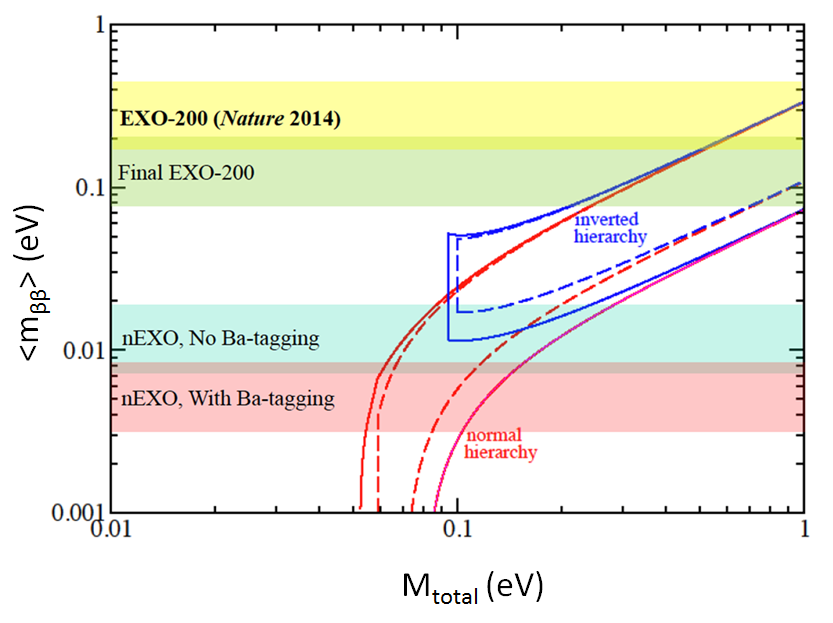
\includegraphics[width=0.48\textwidth]{figures/sensitivity.png}
\caption{Projected sensitivity to the Majorana neutrino mass.  {\color{red}There was en email recently about updating this plot...}}
\label{fig:nEXOsensitivity}
\end{figure}

Techniques are under investigation for barium tagging in both liquid and gas time projection chambers (TPCs).  Progress on a technique for extracting a single ion from a gas TPC and moving it to a trap for detection is described in \cite{Brunner2015}.  Here, we are interested in a technique for barium tagging in the nEXO liquid xenon (lXe) TPC, wherein a cryogenic probe would be moved to the position of the $0\nu\beta\beta$ candidate in order to freeze the daughter ion into a small amount of sXe at the end of the probe.  It would then be detected by its laser-induced fluorescence in the sXe, a technique known as matrix isolation spectroscopy.  Progress for another possible technique for barium tagging from lXe, using resonant ionization of the Ba after it is grabbed on a surface, is reported in \cite{Twelker2014}.

It is expected that a Ba\textsuperscript{++} ion will neutralize once to Ba\textsuperscript{+} in lXe due to ionization potentials [ref], and the dynamics of ionized charge in the lXe following a decay can also result in single or double neutralization.  A new study of neutralization of alpha decay daughters in the EXO-200 lXe TPC, nEXO's predecessor, is in the process of publication [ref from arxiv].  Furthermore, a Ba\textsuperscript{+} ion may neutralize when it is grabbed in sXe in a cold probe.  We are still interested in the feasibility of tagging single Ba\textsuperscript{+} ions as well as single Ba atoms, but we focus here on the latter.

\section{Apparatus}

The apparatus for depositing and observing Ba/Ba\textsuperscript{+} deposits in sXe is described in detail in \cite{Mong2015}, but we describe it briefly here.  Important components are shown in Fig. \ref{fig:apparatus}.

\begin{figure}
\includegraphics[width=0.48\textwidth]{figures/cryo_inkscape_chris_getterwire.eps}
\caption{Experimental setup for depositing Ba/Ba\textsuperscript{+} in sXe matrices, and for excitation and observation.}
\label{fig:apparatus}
\end{figure}

The main source is a Ba\textsuperscript{+} ion beam at 2000~eV, filtered to select Ba\textsuperscript{+} with an E$\times$B velocity filter.  A set of pulsing plates allows 2-$\mu$s pulses for depositing small numbers.  With typical ion currents of 30 - 40~nA, a few of these pulses deposits an ion density sparse enough to resolve single atoms without microscope objective resolution.  Neutralization of the Ba\textsuperscript{+} ions in the sXe matrix makes the ion beam an effective source for Ba in sXe.

An alternative source of neutral Ba is a getter which can be inserted to emit toward the sample.

Deposits are made on a cold sapphire window.  Sapphire has good thermal conductivity at low temperatures, and has modest fluorescence, due to impurities such as Cr\textsuperscript{3+}, which can be largely filtered out in our region of interest.  Sapphire is also extremely transparent, and the 45$^{\circ}$ angle allows access of the Ba\textsuperscript{+}/Ba deposit, as well as of the excitation laser and imaging optics.  

The excitation laser is a Coherent 599 cw dye laser with Rhodamine 6G dye, pumped by the 514-nm line of a Lexel 3500 argon ion laser.  

The first element in the imaging optics is a 50~mm Nikon camera lens.  This collects and collimates the Ba fluorescence.  In the collimated light path, a band-pass filter with FWHM of 20~nm is placed to select the 619-nm fluorescence peak.  A 200~mm Nikon camera lens then focuses the image onto a liquid nitrogen cooled CCD, resulting in an image of 4x magnification.

\section{Method}

Several emission lines observed from neutralized Ba\textsuperscript{+} deposits in sXe are described in \cite{Mong2015}, which are attributed to emission of Ba atoms occupying different Xe matrix sites.  Strong peaks are observed at 577 and 591 nm, as well as others, but a breakthrough in observation of small numbers of atoms comes through observation of the peak at 619 nm.  Decay of fluorescence signal with laser exposure, generally called bleaching, is shown in \cite{Mong2015} to significantly reduce the 577- and 591-nm (and other nearby) peaks within the first few hundred excitations/atom.  These rates are similar to the known rates for optical pumping of Ba into the metastable $6s5d$ states in vacuum.  However, the 619-nm peak does not exhibit bleaching on the time scales in \cite{Mong2015}, and in section \ref{sec:results} we demonstrate signals lasting at least six orders of magnitude longer than that of the 591-nm, etc {\color{red}(should we show this explicitly?)}.  Though less prominent in the first few hundred excitations, the longevity of the 619-nm signal makes it interesting for detecting single atoms.

In \cite{Mong2015} we presented an image of neutral Ba in sXe resulting from about 10\textsuperscript{4} Ba\textsuperscript{+} deposited in the laser region (i.e., $\leq 10^4$ Ba atoms; ions deposited provides an upper limit on the number atoms, as we do not know the fraction of neutralization nor the fraction populating each site), using a band-pass filter which passes only light from the 577- and 591-nm emission peaks.  As mentioned, the limiting factor for these peaks is the fast bleaching rate.

The excitation spectrum for the 619-nm peak is shown in Fig. \ref{fig:excitspec}.  Though not at the peak of excitation, we use an excitation wavelength of 570 nm to maximize the signal to background ratio, where our background comes from a broad emission of Cr\textsuperscript{3+} in the sapphire window.

\begin{figure}
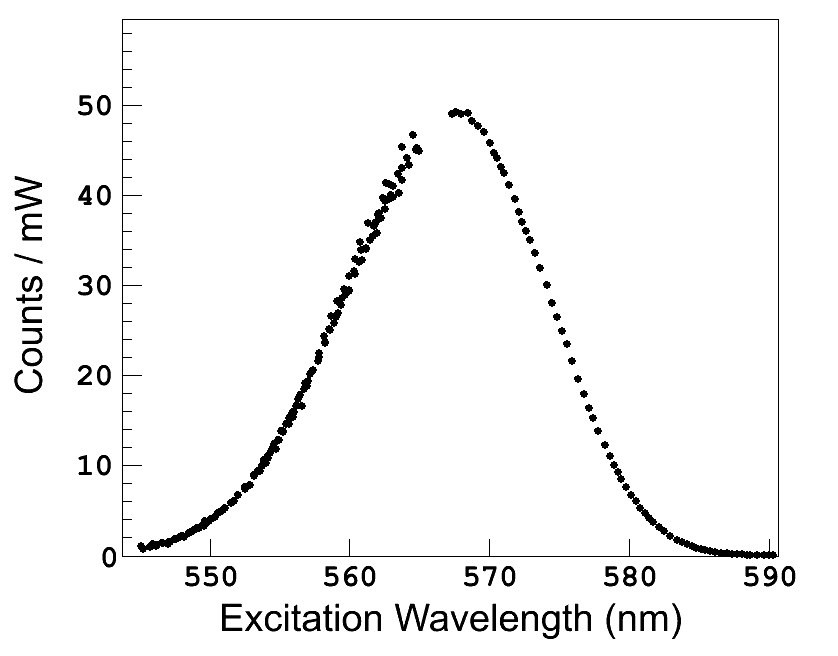
\includegraphics[width=0.48\textwidth]{figures/excitspec.png}
\caption{Excitation spectrum for the 619-nm peak.  The discontinuation is due to use of different laser dyes; lower-wavelength points are obtained with Rhodamine 110, higher-wavelength from Rhodamine 6G.  R110 points are scaled down to the level of the R6G due to different experimental parameters, but overall magnitudes are arbitrary.}
\label{fig:excitspec}
\end{figure}

Samples are created as follows.  Xe gas is directed toward the window using a leak valve, which begins freezing to form the sXe matrix.  This is initiated a few seconds prior to the Ba deposit, continues during the Ba deposit, and is turned off a few seconds after the Ba deposit.  

In this work, deposits are made with the sapphire window at around 50~K. This accomplishes (a) higher 619-nm signal, likely due to a higher population of 619-nm matrix sites, and (b) an absence of hydrogen impurities in the matrix, as hydrogen freezes well below 50~K in vacuum.  The window is then cooled further to 11~K for observation.  

Xe deposition rates resulting in around {\color{blue}50~nm/s} also result in a higher population of the 619-nm site (as compared to lower leak rates), while not being so high as to result in a frosty Xe matrix.

\section{Results}
\label{sec:results}

A typical image is shown in Fig. \ref{fig:image_example}.  The focused laser's path through the sapphire window is seen as a semi-vertical line (its orientation depending on mirror angles).  As mentioned, Cr\textsuperscript{3+} impurities in the sapphire produce a broad fluorescence, the tail of which enters the 620 band-pass filter used in these images.  This and another background emission from the window surfaces are discussed further in section \ref{sec:backgrounds}.

\begin{figure}
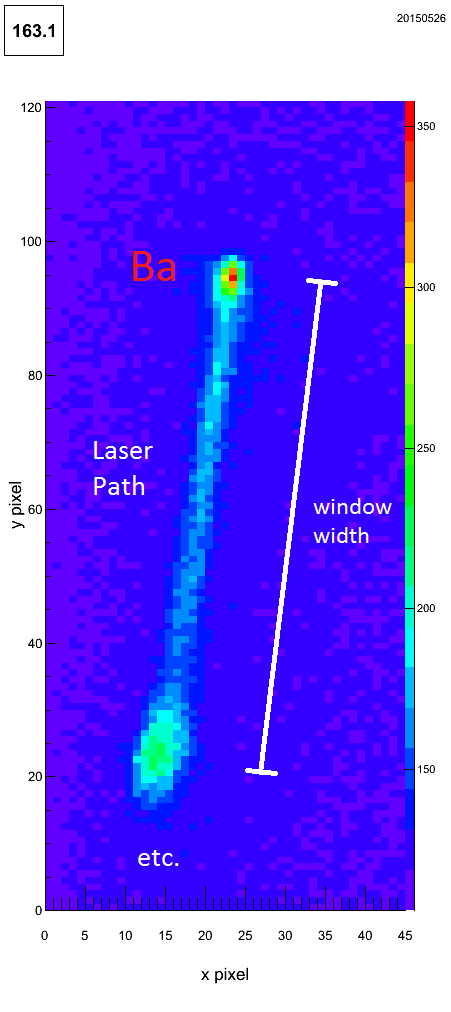
\includegraphics[width=0.3\textwidth]{figures/2015-05-26_163_1.png}
\caption{{\color{red}Maybe this should be combined with Xe/Ba/Xe image.}}
\label{fig:image_example}
\end{figure}

A Ba\textsuperscript{+} deposit covers an area much larger than this, but we only observe fluorescence from those atoms (neutralized ions) which are in the laser region.  Since the Ba\textsuperscript{+} lands only on one surface of the window, it appears in the image as a peak at one end of the laser path.

By knowing the size of the laser region, as well as the density of ions deposited per pulse, we can determine the upper limit on the number of atoms in a deposit.  The minimum laser focus $w_0$ is measured in air, and calculated to be about {\color{red}3~$\mu m$ (\textbf{mention astigmatism?} Worry about the discrepancy between measured and calculated distance between x and y focus?  Someone should reproduce that.)} in the sapphire, and subsequently in the thin layer of sXe.  This results in about 0.06 ions/pulse deposited into the 1/e radius of the laser region for 13~fC/pulse of the ion beam.

In an experiment, a deposit is made and observed, and then evaporated by heating the window to 100 K.  Many deposits are observed, with varying numbers of ion pulses, in order to demonstrate (a) linearity in observed signal vs. the number of atoms, and (b) repeatability/stability of deposits.  To ensure that no Ba is left over from previous deposits, Xe-only runs (where the Ba\textsuperscript{+} beam is deflected and blocked by the Faraday cup) are done frequently in between Ba\textsuperscript{+} deposit runs.  This also provides a local background image for each Ba image.  Fig. \ref{fig:raw}b shows a $\leq$ 3-atom deposit (3 ions deposited) with Xe-only deposits made before and after (Fig. \ref{fig:raw}a,c)).

Fig. \ref{fig:linearity} shows the linearity in summed CCD counts, from the image of the laser region on the sXe surface, vs. ions deposited for several deposits.  Each point has subtracted the counts from a nearby Xe-only run.  We observe about 43~counts/mW per atom with 3-s CCD exposures.

Xe-only images can be directly subtracted to obtain images of Ba fluorescence.  Fig. \ref{fig:lego}(a) shows subtracted images for a range of deposit sizes.  

\begin{figure}[h!tb]
	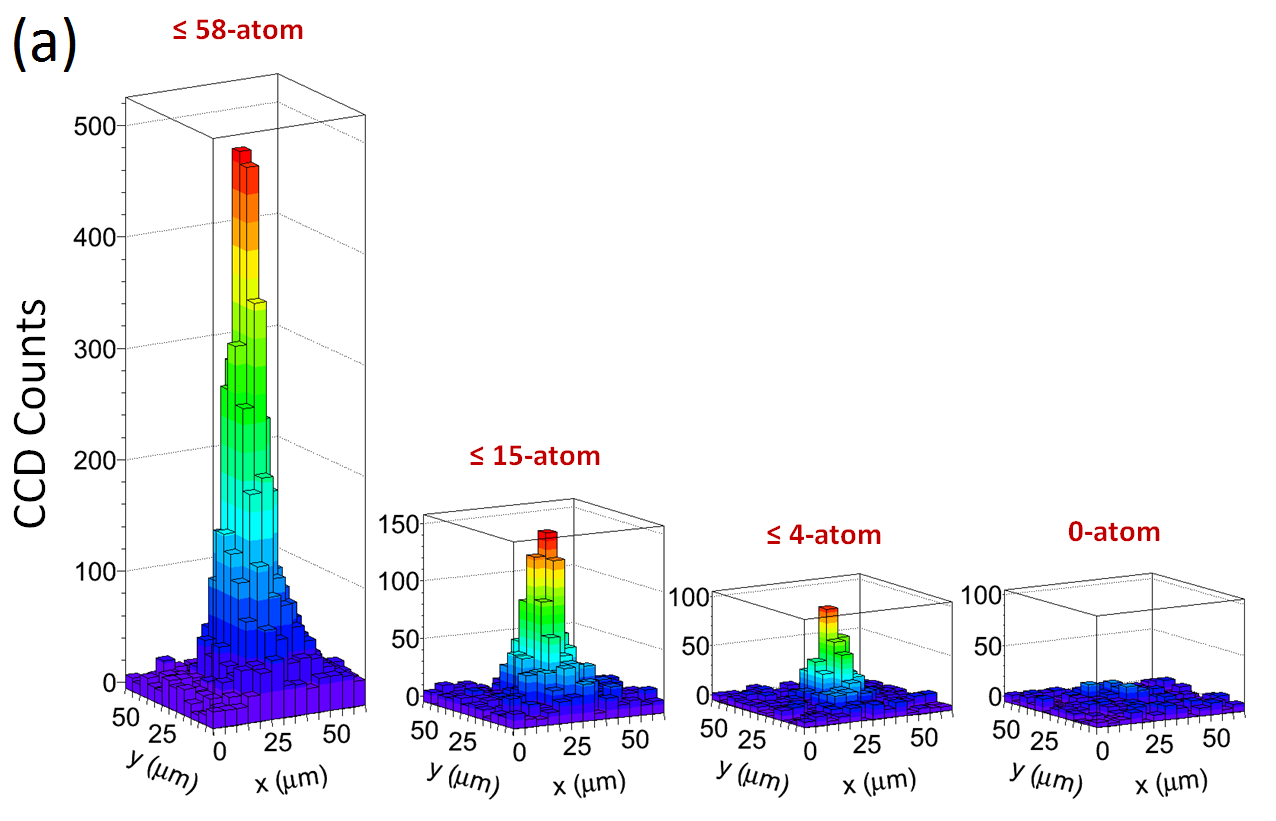
\includegraphics[width=0.45\textwidth]{figures/lego_varying.png}
	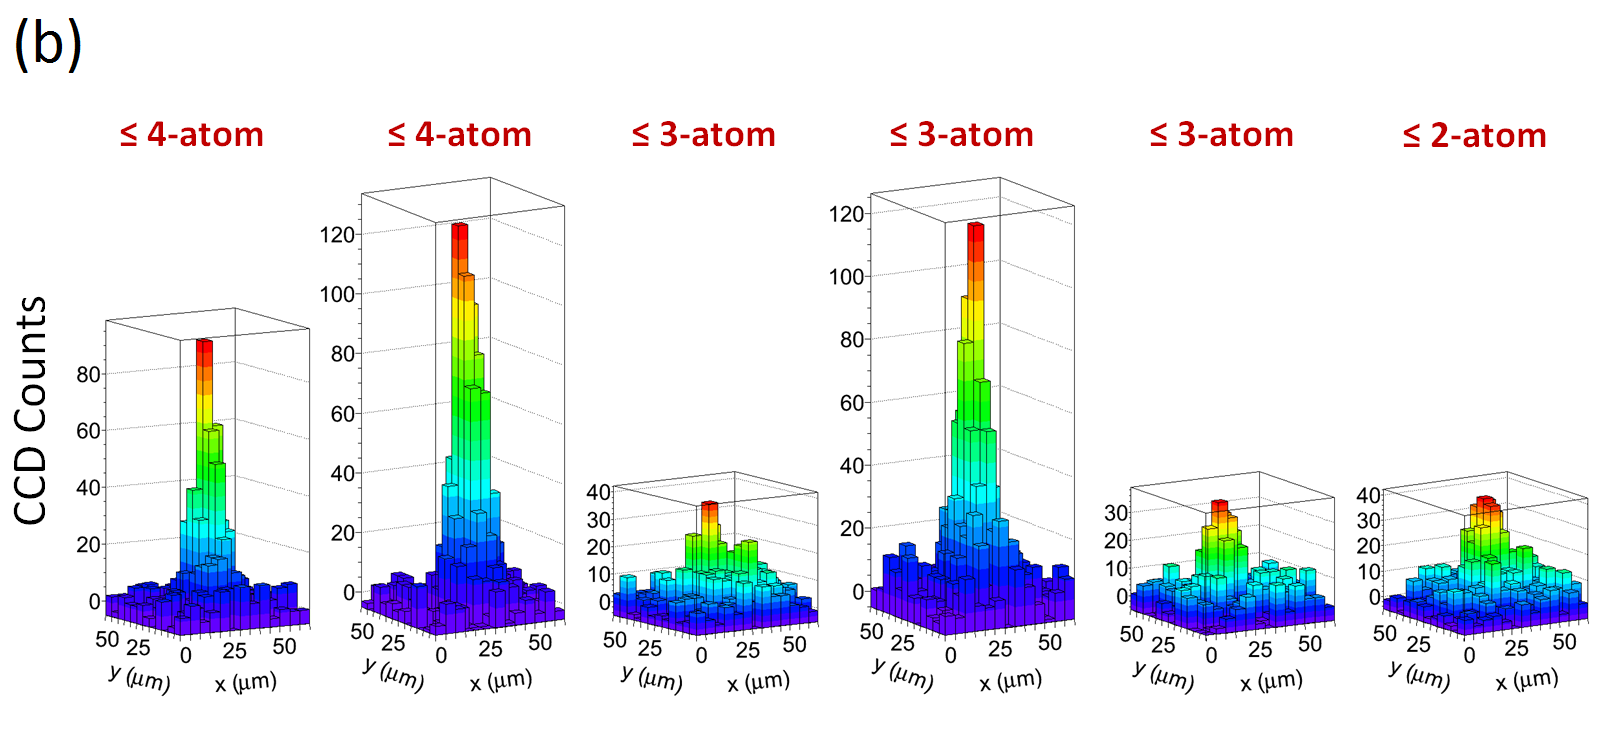
\includegraphics[width=0.45\textwidth]{figures/lego_statistical.png}
	\caption{Direct subtraction to obtain images of Ba fluorescence.  {\color{gray}Maybe refer to uncertainties in linearity plot.}}
	\label{fig:lego}
\end{figure}

Fig. \ref{fig:lego}(b) shows several of the very small numbers deposits.  Poissonian fluctuations will occur on the number of ions landing in the laser region, as well as on where they lie in the Gaussian distribution in the beam, resulting in fluctuations in the observed signal.

The reader will notice that the laser region in the images (each pixel is $5\times5~\mu m$) appears about 4~x larger than the calculated {\color{red}3-$\mu m$} $w_{0}$.  This is partly due to the maximum resolution of the collection optics, and partly due to vibrations between the laser and the collection optics at the 2- to 3-$\mu m$ level.

There is also a relative vibration between the cryostat and the laser/collection optics which is important to understand, caused by vibrations of the pumping mechanism in the cryostat.  This vibration does not cause blurring of the image, but results in slight movement (3- to 4-$\mu m$ level) of the laser over different regions of the deposit.  The signal at a given time is coming from ($\leq$) the calculated number of atoms, but they are not from the same individual atoms at all times.  {\color{red}(Maybe this should be mentioned more at the beginning.)}

\begin{figure}
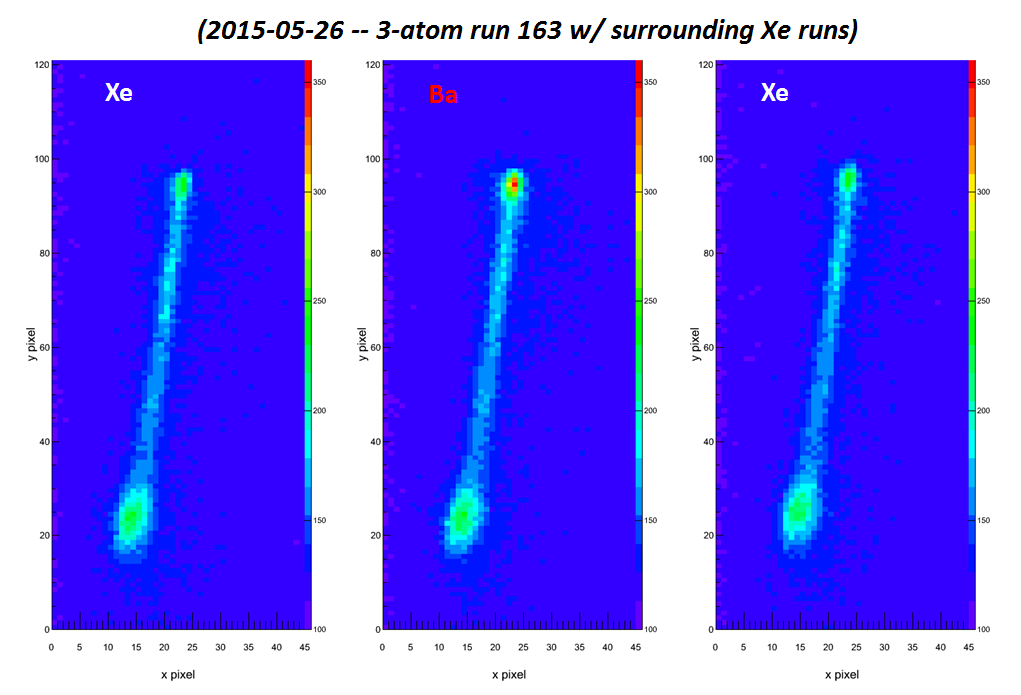
\includegraphics[width=0.48\textwidth]{figures/image_raw_3-atom_with_pre-post-.png}
\caption{caption}
\label{fig:raw}
\end{figure}

\begin{figure}
\includegraphics[width=0.48\textwidth]{figures/linearity.png}
\caption{Linearity of 619-nm Ba fluorescence vs. number of ions deposited.  {\color{red}should x-axis be Ions Deposited in Laser Region ($\leq$)?  Talk about uncertainties here -- x-axis is from laser spot size and from ion deposit}}
\label{fig:linearity}
\end{figure}

Fig. \ref{fig:anneal} shows the temperature dependence of the 619-nm fluorescence.  It is all but gone at 42~K, but its return when re-cooled indicates loss of fluorescence efficiency at the higher temperature, not loss of the Ba atoms to chemical reactions or evaporation.  An overall loss after warming to the higher temperature of 48~K indicates some loss of the atoms.

This temperature dependence of the fluorescence means that the probe in nEXO will need to be moved to a location out of the lXe where it can be cooled to 10 - 15~K.

{\color{gray}This could be in a subsection about the proerties of the matrix site, since we might also want to talk about the annealing of a 10~K deposit increasing the signal, and maybe have figures showing the higher signal with 50~K deposits and with higher leak rates (this interesting but is kind of separate from imaging).  This stuff is mentioned in Method.}

\begin{figure}
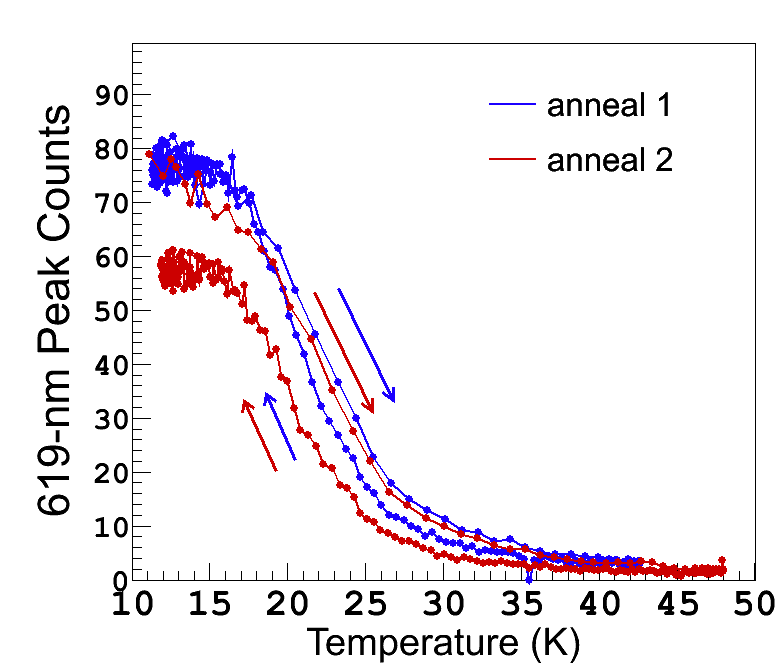
\includegraphics[width=0.48\textwidth]{figures/paper_single-atom_619-anneal_20150916_runs36and37_omitRun34_arrows.png}
\caption{Observing 619-nm peak through annealing process.  Lower fluorescence is observed at higher temperature, but essentially no signal is lost after returning to 10~K in anneal 1.  This demonstrates the stability of the site.  Anneal 2, to higher temperature of 48~K, does result in loss of overall signal.  {\color{red}[This omits the actually first anneal, which is of a 10~K deposit, so it shows an \emph{increase} in signal -- this is interesting, but maybe confuses the plot.  It goes more w/ why we deposit at 50~K...]}}
\label{fig:anneal}
\end{figure}

\subsection{Identification of 619-nm Peak as Ba in sXe}

{\color{gray}\emph{should this be in Discussion?}}

Several tests have aided in identifying the 619-nm peak as pure Ba in sXe.  Firstly, a molecule of more than one Ba is ruled out by a high Xe/Ba ratio.  Our ion currents and Xe deposition rates result in around 10\textsuperscript{4}:1 for this ratio, 10~x higher than the recommended ratio in [ref that old paper].

Secondly, the observation of the 619-nm fluorescence with deposits made from the purely neutral Ba source, the getter wire.  Fig. \ref{fig:ion_getter_ar} shows the identical shapes of the 619-nm peaks from Ba getter and Ba\textsuperscript{+} ion deposits.  Observing Ba in this 619-nm matrix site at the low-energy (thermal) deposit from the getter is also good news for the prospect of grabbing Ba/Ba\textsuperscript{+} on a probe out of lXe at low energy.

\begin{figure}
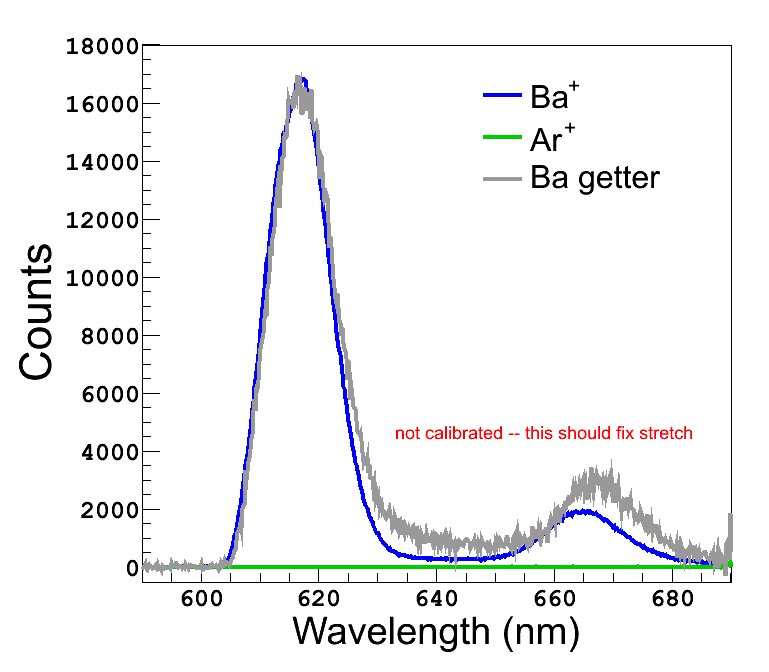
\includegraphics[width=0.48\textwidth]{figures/getter_ion_Ar.png}
\caption{caption}
\label{fig:ion_getter_ar}
\end{figure}

Fig. \ref{fig:ion_getter_ar} also shows the absence of the fluorescence when Ar\textsuperscript{+} is deposited into sXe under the same conditions.  This rules out any matrix-damage-related sources of the 619-nm peak, such as F-centers, which in principle could be created by ionized electrons binding to matrix vacancies.  

{\color{red}I'm having trouble re-producing this, so maybe we leave it out:  }{\color{gray}Finally, a measurement of the Ba\textsuperscript{+} beam velocity confirms a mass of $137(?) \pm ?$, ruling out any contribution of barium oxide }(But probably not BaHx\textsuperscript{+}){{\color{gray}in the beam.  This is possible by knowing (a) the energy of the ions (2000~eV), (b) the time between the signals in a set of induction plates and the Faraday cup as well as the distance between the two, and (c) the timing of those signals for a pulse of Ar\textsuperscript{+} at the same energy, whose mass we know.  }

\section{Discussion}

It is worth noting that the initially lower amplitude of the 619-nm peak, vs. the peaks around 590~nm, does not imply anything about their relative populations.  Different matrix sites can have very different effects on electron transition rates, and fluorescence efficiencies can be quite different.  In fact, the fluorescence efficiency of the 619-nm site is measured to be {\color{red}$1\times10^{-5}$}, calculated using the cross section of Ba in sXe reported in \cite{Mong2015}.

\subsection{Backgrounds}
\label{sec:backgrounds}

Background in the images come from any additional light in the 610-630~nm region, which is passed by the band-pass filter.  As mentioned, Cr\textsuperscript{3+}, an impurity in sapphire, emits a small amount of broad fluorescence, which produces the image of the laser path in the window and results in a modest background for single-atom detection.  More well-known will be the sharp, strong emission peaks of Cr\textsuperscript{3+} in sapphire around 693~nm (used in ruby lasers).  These lines are filtered out.  We identify the broad emission as also due to Cr\textsuperscript{3+} by an identical excitation spectrum.  This background has been mediated by using the highest purity of sapphire windows commercially available from companies like Meller Optics and Rubicon Technologies.

Another background is observed on the surfaces of the window, also caused by laser excitation.  This is more of a nuisance, as it not as easily distinguished from the Ba in an image.  It also exhibits bleaching, which can cause confusion in subtractions, though its bleaching rate is different from that of the 619-nm Ba emission.  

The surface background becomes brighter as the sapphire window is cooled, increasing steadily immediately from room temperature, suggesting that it is due to residual gases which steadily freeze on the surfaces {\color{red}(it levels off around 100~K ... does this suggest that it's actually just a temperature-dependent fluorescence instead of something steadily freezing, or would it happen by a maximum coating thickness and/or a depletion of gases in the vacuum?)}.  Its bleaching could be attributed to evaporation or annealing by laser heating, or by optical pumping into metastable states {\color{red}(do we want to mention Kr repump as suggesting the latter?)}.

The set of deposits used for Fig. \ref{fig:linearity} was done after significant pre-exposure of the sapphire window to the focused laser, bleaching the surface background to a low, constant value which interfered minimally with small-number deposits.

However, it has been observed that Ba\textsuperscript{+} deposits made on a pre-bleached surface result in a somewhat {\color{red}(Is this well-developed enough, or even worth mentioning?)} lower efficiency of 619-nm signal, at about 75\%.  This could be due to a different Xe matrix structure on a surface of annealed or evaporated frozen gases.  Note that this is a very thin layer of frozen residual gas -- interference fringe experiments have put limits on its thickness to $\leq$ 0.02~nm/s ({\color{red}would we expect residual gases to make a nice enough matrix for fringes?}) \textbf{\color{red}\emph{This is based on 7000~s of no fringe observed on initial-freeze residual gas fringe search, but maybe we want to do this as the cryo is cooling, not when it is cold}}.

Note that backgrounds due to impurities are not expected in the high-purity lXe environment of nEXO.

\section{Conclusions}

The 619-nm emission peak observed in deposits of Ba\textsuperscript{+} and Ba in sXe is attributed to neutral Ba a stable and relatively abundant matrix site.  An excitation spectrum and temperature dependence of the fluorescence are reported.  Images of 619-nm fluorescence in a focused laser region from Ba atoms are achieved down to an average number of Ba atoms at the single-atom level.

Successful detection of Ba atoms at this level, with very different energies of deposit, is a significant step toward the development of the Ba tagging technique for the nEXO lXe TPC.  

\section*{Acknowledgements}

Shon Cook and Brian Mong for pioneering work and primary authorship in \cite{Mong2015}.  This material is based upon work supported by the National Science Foundation under Grant Nunber PHY-1132428 and the U.S. Department of Energy, Office of Science, Office of High Energy Physics \textbf{\textcolor{red}{under Award Number DE-FG02-03ER41255.}}

%\bibliography{references10}
\begin{thebibliography}{00}

\bibitem{Mong2015} B. Mong \emph{ et al.}, Phys. Rev. A \textbf{91}, 022505 (1954).

\bibitem{Twelker2014} K. Twelker \emph{ et al.}, Review of Scientific Instruments \textbf{85}, 095114 (2014).

\bibitem{Brunner2015} T. Brunner \emph{ et al.}, International Journal of Mass Spectrometry {\color{red}\textbf{379} (2015) 110-120.}

\end{thebibliography}

\end{document}